\documentclass[12pt,a4paper]{article}
\usepackage{graphicx}
\usepackage{array}
\graphicspath{ {/} }
\title{Cross-Plaform Application Development using React Native}
\author{ Sanket Sabale }
%\date


\begin{document}


\maketitle
\newpage
\tableofcontents
\newpage




\section*{Abstract}

 React Native is an Open-Source UI software Framework created by Meta Platforms, in 2015. It is Used to Develop Applications for Android and IOS By enabling developers to use React Framework along with native platform capabilities. It is also being used to develop virtual reality applications at Oculus. The Working Principle of React native are virtually identical to React except that React Native does not manipulate the DOM via the Virtual DOM. It runs in a background process (which  interprets the JavaScript written by the developers ) directly on the end-device and communicates with the native platform via serialized data over an asynchronous and batched bridge. React Components wrap existing native code and interact with native API’s via React’s declarative UI paradigm and JavaScript. While React native styling has a similar sytax to css it does not use HTML or CSS. Instead, messages from the JavaScript thread are used to manipulate native views. React Native also allows developers to write native code in languages such as Java or kotlin for Android, objective-c or swift for ios, and C++/WinRT or  for Windows 10, Which makes it even more flexible Microsoft builds and maintain React Native for windows and React native for macOs.

\addcontentsline{toc}{section}{Abstract}

\newpage

\section*{Motivation}

Today React Native is Accepted By Many Different Companies and They are Hiring React Native Developers . \\
\begin{figure}[h]
    \centering
    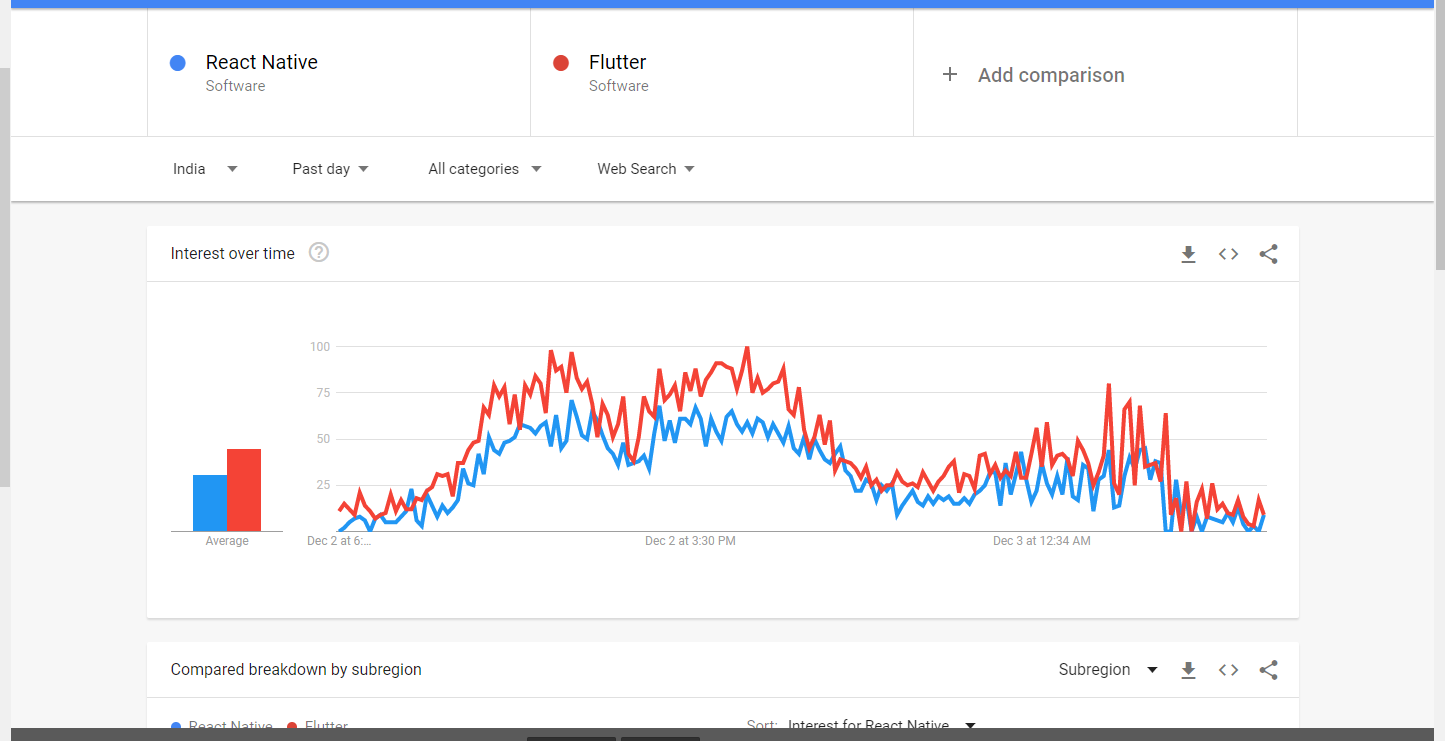
\includegraphics[width=0.55\textwidth]{react_trends}
\end{figure}
\\
 \qquad Also React Native is doing a greate job to beat the other alternatives.We all know that Android users are huge as compare to another platforms and thats why there are millions of apps are downloaded every day so demand of an android developers are really big so if you are wanted to become an android developer you need to pick a perticular android technology but if you have knowledge of web development like JS,HTML,CSS and ReactJS You can Continue with it and you can master these development with React Native. It is a Greate Platform who can give you authority to write code once and make or convert it in IOS and Android App so you don't need to write code for android and ios differently so the big problem are going to be fixed up here. React Native is really gone to easy who are in web development you can connect any backend framework to the android app which is build with react native also there are few other tech as well where you can connect backend but in react native it is easy to connect.

\addcontentsline{toc}{section}{Motivation}
\newpage

\section*{Literature Survey}
\addcontentsline{toc}{section}{Literature Survey}
\subsection*{React Native Based Mobile App for Online Experimentation}
\addcontentsline{toc}{subsection}{React Native Based Mobile App for Online Experimentation}
\begin{tabular}{ |c | m{2.5cm} | m{2cm}| c | m{2cm} | m{2cm} | c | }

  \hline
  sr.no & Title of Page & Author & Published Year & Finding & Future Scope  \\ 
  \hline
  1 & React Native Based Mobile App for Online Experimentation & Xingwei Zhou etal. &  2020 & IEEE Xplore & Helps Student To  get Practicle Exprerince Through 3D \\
\hline 
  
\end{tabular}
\\
\\
\\
In These Article We Found That Author is Telling us That How a Laboratory can be an online tool for everyones use by react native so basically The Concept is there are so many collages which don't have 
practical lab so we can create an app for those student so that he can practice on 3D images and Touchable Effects its looks similar to real practice in it so we can solve a problem of Practical labs in all collages but there some things That i like to update is that we can improve thos UI for students and every single branch needs there own space for practice it also we can include some of test exams so that teacher can see knowledge of student or What he gain? so far.
\\
\\
\newpage
\subsection*{React Native Supplements}
\addcontentsline{toc}{subsection}{React Native Supplements}
\begin{tabular}{ |c | m{2.5cm} | m{2cm}| c | m{2cm} | m{2cm} | c | }

 \hline
  sr.no & Title of Page & Author & Published Year & Finding & Future Scope  \\ 
  \hline
  2 & React Native Supplements & Paul etal. &  2019 & Springer & Guide For Developers \\
\hline 
  
\end{tabular}
\\
\\
\\
These Article is written for help to understand the backend code of React Native. In these Reflux Patterns are explained in very different and Easier manar so that if react native developers whants to implement somethings they get help from these pattern not only these article also tells about Redux the big state management tools to manage states Many of the industries are actually working on it.
So These Articles also tells about how to use redux? How the you can debugg your apps in android phone using deugging mode. But we can implement some libraries for easy development and we can import statements to import more packets. There are lots of things are covered in these article and its helpfull when wants to understand React native deep concepts but for now we have lot more libraries that comes with pre-builted code that help us to us functionality directly on our App.


\newpage
\subsection*{Mobile Development in Swift, Java and React Native}
\addcontentsline{toc}{subsection}{Mobile Development in Swift, Java and React Native}
\begin{tabular}{ |c | m{2.5cm} | m{2cm}| c | m{2cm} | m{2cm} | c | }

  \hline
  sr.no & Title of Page & Author & Published Year & Finding & Future Scope  \\ 
  \hline
  3 &  Mobile Development in Swift, Java and React Native & Hugo Brito etal. &  2019 & IEEE Xplore & Comparing Technologies \\
\hline 
  
\end{tabular}
\\
\\
\\
We know that there are so many technologies are present in the market for creating Android and IOS apps but which is best and how we can found it? The perticular question is solved in these article. while we are creating a Native App we are using Java For android and swift for IOS and to create a both platform application we are using React Native. In native application we found that the performnce of it is really good as compaire to react native but to use more and different library  we need to write to much heavy code and these may be possible that library not presented so we need to manage lots more things to get that functionality done in native apps so that React native solve our problem my suggestion will be like go for react native its saves your time for writing the code which already present and we can compair with these react native with some more cross-plaforms like flutter  and Ionic.

\newpage
\subsection*{JavaScript in Mobile Applications: React native vs Ionic vs NativeScript vs Native Development}
\addcontentsline{toc}{subsection}{JavaScript in Mobile Applications: React native vs Ionic vs NativeScript vs Native Development}

\begin{tabular}{ |c | m{2.5cm} | m{2cm}| c | m{2cm} | m{2cm} | c | }

  \hline
  sr.no & Title of Page & Author & Published Year & Finding & Future Scope  \\ 
  \hline
 4 &  JavaScript in Mobile Applications: React native vs Ionic vs NativeScript vs Native Development & Anabela Gomes etal. &  2018 & IEEE Xplore & Comparing Technologies \\
\hline 
  
\end{tabular}
\\
\\
\\
These Article Also Compare React native with other technologies but Its Compare with cross-platforms mean the other platforms also work as like a react native and by these comparison we are getting best idea to which tech is used for what kind of projects? and you can pick a grate platform. In lot more cases the tech you pick is not suitable for that perticular project may be the other tech performs better then your's in that case you need to use another tech for it that explaination is inside these article but my opinion will be to improve or add other platforms to like flutter and again compare with it because flutter is also a greate tool it usages a dart programming language and its more over an object oriented programming language  so the code you are writing is in classes and object its not a functional base thats the big disadvantage of flutter but its also quite popular in the market now.

\newpage
\subsection*{Exploration of React Native Framework in designing a Rule-Based Application for healthy lifestyle education}
\addcontentsline{toc}{subsection}{Exploration of React Native Framework in designing a Rule-Based Application for healthy lifestyle education}

\begin{tabular}{ |c | m{2.5cm} | m{2cm}| c | m{2cm} | m{2cm} | c | }

  \hline
  sr.no & Title of Page & Author & Published Year & Finding & Future Scope  \\ 
  \hline
 5 &  Exploration of React Native Framework in designing a Rule-Based Application for healthy lifestyle education & Anik Hanifatul Azizah etal. &  2021 & IEEE Xplore & Lifestyle and Education \\
\hline 
  
\end{tabular}
\\
\\
\\
As  we know in these world is Going to faster tech world and now healthy lifestyles is going to be little bit hard for us to find so that these article tells us how we can live a helthy life styles using React Native Rule-Based Application these application comes with some basic rools so that excising and drinking and some more task can be done throught out the notification functionality and some more functionality so that lifestyle becomes technical healthy. But After read these article i think that there are more things we can improve on to it like exerise videos and basic audio file for stress free brain and some more things but all the way these is greate things to work on it and for the healthy lifestyle these ideal is greate to work on it.

\newpage
\section*{Problem Statement}
\addcontentsline{toc}{section}{Problem Statement}
\subsection*{What is Problem?}
\addcontentsline{toc}{subsection}{What is Problem?}
\qquad In real industries we found that when application project started client requirement is App should be work on cross-plaforms means it can able to run on android as well as ios devices so if you try to understand this thing is little bit complecated for development first developers needs to write code for android and then he also need to write there codes for ios in both different languages so company need to hire developers for android as well as ios so that he can complete the clients project in efficient manor but some how the features which you see in IOS not available in Android in that case android app become littel bit different from ios app not the UI but feature are different and thats the big reason for big compnies are switching to cross-platform development I am not saying that cross-platform is best that other native platforms there is advantages  of native platforms as well but with the cross-platform application companies can save his time also they don't need hire different developers for different platforms so its saves money as well. There are some Companies who are working on native platforms as well because not every client say i need cross-platform apps some clients are only need android app to be developed in that case to make app more fast companies prefer to go for native platforms like Kotlin or Java. Also Same as IOS developers they work on objective-c and Swift for creating apps for IOS devices so companies are also hire them as well now why companies is are hiring native developers? if the cross-platform technology is here? as i said native apps have there own advantages like you can customize everything which you like and create interface as you want. but in cross-platform development there are so many things are already customized for you so you can't change it, but the feature its provide is really good for designing it can create better UI as compare to Native apps ( It's my Personal Exeperience ) so Now Problem is How React Native can Solve our Problem? Is it Can or Not.

\newpage

\subsection*{How React Native is Works?}
\addcontentsline{toc}{subsection}{How React Native is Works?}
\qquad React Native is based on ReactJs Framework library its quite become popular when ReactJS cames into the market right there so many software developers like to use ReactJS as Frontend Framwork but right we are on React Native Side. React Native compiles the JavaScript code to native components, thus, using platform-specific APIs and modules. By using such native components as Images, Text, and View as building blocks, software developers can create new ones.
React Native allows the development of apps consisting of JS code and native by making the bridge between an app and a target platform. When JavaScript has been running along with some native code, the React Native’s bridge system leverages the React library and transfers components’ hierarchy to the mobile device view. In case of any updates, for example, if a user presses the button, React Native translates this case into the event that the JS can handle. And then, by relaying messages between a particular native platform and a JS codebase, the React Native bridge translates native events into ones React components can understand and respond to. Being single-threaded, React Native apps are easy to understand since everything that works with JavaScript on the web, will work the same way on React Native. But it’s important to consider JS specifics while developing an app architecture in order to avoid performance issues. If the architecture of the future app involves many events and a lot of data, React Native app development may not be the best option since the bridge structure may cause delays. But Due to the bridge architecture, some long-running events on the JS side may block UI events. Also, any actions requiring synchronization between JS code and native one may be delayed because of the time required to pass information via the bridge. For example, there might be issues with a ScrollView’s position since events about its change are rapidly emitted.
\par
Performance of React native is might be not good at some cases due to single threading architechture but there are more ways to solve these problem and we can do faster things in it as well. Talking about the interactive animations, that should run every 16 milliseconds, their logic goes from the JS to the Native side. Due to bridge architecture, animation events may also have performance issues. When developing React Native-based apps, we used Native Driver, which sends animations to the native side. The native code performs animations in the UI thread which allows frames to avoid going through the bridge and ensures smoother performance. 






\end{document}